%! Author = gramic
%! Date = 08.04.24

% Preamble
\begin{flushleft}
    \subsubsection{Evaluation - Testfälle}
    \paragraph{Patroni}
    \begin{description}
        \item \textbf{Failover}\hfill \\
        \begin{enumerate}
            \item Der Server des primäre Node wird manuell heruntergefahren.
            \item Während des Failover müssen Daten via SQL\\eingeführt und ausgelesen werden.\\Testskripte müssen sollen als Batch-Job ausgeführt werden.
            \item Während des Failover muss mindestens eine längere Abfrage gestartet werden.
        \end{enumerate}
        \item \textbf{Switchover}\hfill \\
%        \setcounter{enumi}{4}
        \begin{enumerate}[resume]
            \item Mit der REST-API wird der Switchover\\auf einen anderen Nod abgesetzt.
            \item Mit dem \texttt{patronictl}-Command wird der Switchover gesetzt
            \item Während dem Switchover müssen Daten via SQL\\eingeführt und ausgelesen werden.
            \item Während dem Switchover muss mindestens eine längere Abfrage gestartet werden.
        \end{enumerate}
        \item \textbf{Restore}\hfill \\
%        \setcounter{enumi}{9}
        \begin{enumerate}[resume]
            \item Mit der REST-API wird der Node erst mit dem \texttt{reinitialize} wiederhergestellt\\und dann mit einem Switchover wieder als Primary gesetzt.
            \item Mit dem \texttt{patronictl}-Commandund Parameter \texttt{reinit} der Node wiederhergestellt\\und abschliessend mit Hilfe Switchover wieder als Primary gesetzt.
            \item Mit der REST-API wird der Node mit dem \texttt{reinitialize} wiederhergestellt
            \item Mit dem \texttt{patronictl}-Commandund Parameter \texttt{reinit} der Node wiederhergestellt
            \item Vor, während und nach dem Restore müssen Tabellen mit Foreign-Key-Constraints und Daten geprüft werden.
            \item Während des Restore muss mindestens eine längere Abfrage gestartet werden und Daten via SQL\\eingeführt und ausgelesen werden.
        \end{enumerate}
    \end{description}
    \paragraph{StackGres - Citus}
    \begin{description}
        \item \textbf{Failover}\hfill \\
        \begin{enumerate}
            \item Der Server des Leader-Cooordinator-Node wird manuell heruntergefahren.
            \item Während des Failover müssen Daten via SQL\\eingeführt und ausgelesen werden.
            \item Während des Failover muss mindestens eine längere Abfrage gestartet werden.
        \end{enumerate}
        \item \textbf{Sharding}\hfill \\
%        \setcounter{enumi}{4}
        \begin{enumerate}[resume]
            \item Vor, während und nach dem Failover müssen Tabellen mit Foreign-Key-Constraints geprüft werden.
            \item Nach einem Failover-Test müssen alle Daten vorhanden sein.
        \end{enumerate}
        \item \textbf{Self Healing}\hfill \\
        \begin{enumerate}[resume]
            \item Der Node muss wieder hochgefahren werden.\\Der Node muss selbstständig Daten synchronisieren.
            \item Der Leader muss, falls notwendig, automatisch neu gesetzt werden.
        \end{enumerate}
    \end{description}
    \paragraph{YugabyteDB}
    \begin{description}
        \item \textbf{Failover}\hfill \\
        \begin{enumerate}
            \item Ein k8s Node wird manuell heruntergefahren,\\indem der entsprechende Server heruntergefahren wird.
            \item Während des Failover müssen Daten via SQL\\eingeführt und ausgelesen werden.
            \item Während des Failover muss mindestens eine längere Abfrage gestartet werden.
        \end{enumerate}
        \item \textbf{Sharding}\hfill \\
%        \setcounter{enumi}{4}
        \begin{enumerate}[resume]
            \item Vor, während und nach dem Failover müssen Tabellen mit Foreign-Key-Constraints geprüft werden.
            \item Nach einem Failover-Test müssen alle Daten vorhanden sein.
        \end{enumerate}
        \item \textbf{Self Healing}\hfill \\
        \begin{enumerate}[resume]
            \item Der Node muss wieder hochgefahren werden.\\Der Node muss selbstständig Daten synchronisieren.
        \end{enumerate}
    \end{description}
\end{flushleft}
\begin{flushleft}
    \subsubsection{Evaluation - ERD self\_healing\_test}
    \label{subsubsec:erd_self_healing_test}
    Die Tests müssen bei allen drei Varianten anhand der Datenbank \texttt{self\_healing\_test} durchgeführt werden.\\
    Dabei werden die Tabellen im Hinblick auf das Citus Schema Based Sharding in Schemas organisiert.\\
    Zwischen den einzelnen Schemas sollen einige Tabellen einen Foreign-Key auf andere Tabellen legen:
    \begin{figure}[H]
        \centering
        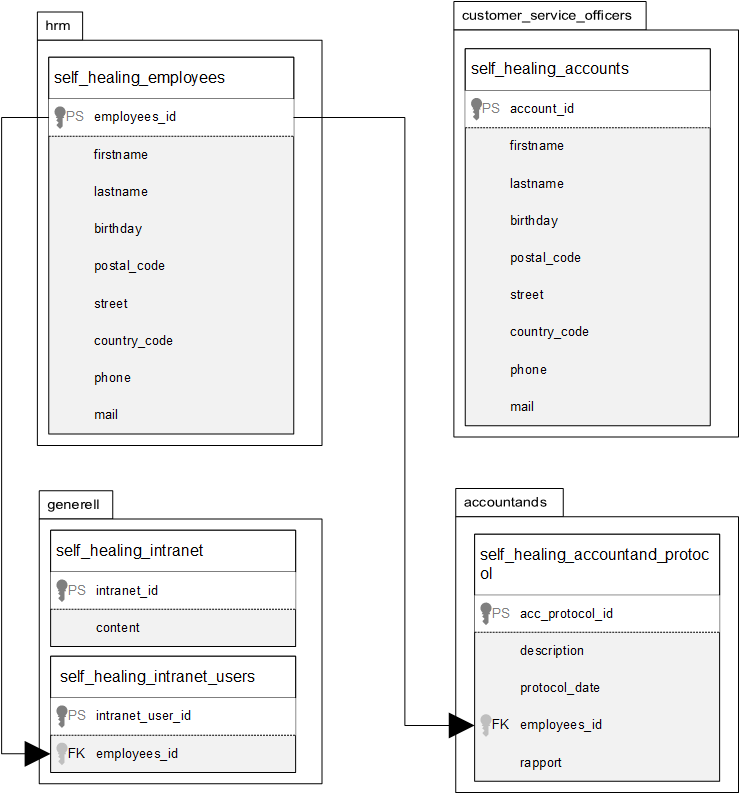
\includegraphics[width=0.5\linewidth]{source/implementation/evaluation/evaluation_tests/erd_self_healing_test}
        \caption{Testing - ERD DB self\_healing\_test}
        \label{fig:erd_self_healing_test}
    \end{figure}
\end{flushleft}